\documentclass[10pt]{article}
\usepackage[margin=0.72in]{geometry}
\usepackage{graphicx,booktabs,tabularx,array,hyperref}
\hypersetup{colorlinks=true,urlcolor=blue}
\title{ECDLP follow-ups: paired factor-base sweep and Kummer addition gate}
\author{Reproducible experiment report}
\date{21 October 2026}
\begin{document}
\maketitle
\noindent\textbf{Scope.} The frozen protocol covers four leads on 21 exact-order
Scholten models, 60 separate targets per model. This report contains completed
factor-base and jump experiments and an exact Kummer applicability gate.
The complete inversion-free law and full-cohort pencil collector remain open.
All costs are cold one-target operation-count prices, not wall-speed claims.

\section*{Factor-base and jump sweep}
Five arms solved and source-verified all 1,260 targets each, with zero failures
or cap exhaustions. All 6,300 same-process rho controls were also source-verified.
All 1,260 incumbent count and phase records replay exactly.
At $M+0.5S+10I$ and 0.1 source-addition equivalents (GAE) per declared native
logical operation, matched negation rho totals 1,088,802,370 GAE.

\begin{center}\small
\begin{tabular}{lrrrr}
\toprule
Arm & Divisors processed & Total GAE & / external & / rho \\
\midrule
Full base, 16 jumps & 219,581,773 & 2,666,291,894 & 1.000000 & 2.448830 \\
Full base, 8 jumps & 220,092,171 & 2,664,487,778 & 0.999323 & 2.447173 \\
Full base, 32 jumps & 219,864,588 & 2,671,135,032 & 1.001816 & 2.453278 \\
Half base, 16 jumps & 282,983,105 & 3,285,713,695 & 1.232316 & 3.017732 \\
Quarter base, 16 jumps & 392,583,830 & 4,267,226,320 & 1.600435 & 3.919193 \\
\bottomrule
\end{tabular}
\end{center}

The half and quarter bases rejected 35,385,164 and 110,402,348 split
relations, respectively, when neither root was in the fixed target-blind
base; all rejected candidates were charged. None of the five arms is below
rho in the 36 pooled pricing cells. The 8-jump arm is below the 16-jump arm
in 15 of 36 cells. Across bit sizes it is below at 16, 20, 24 and 40 bits,
and above at 28, 32 and 36 bits. One seed was used per target; no uncertainty
interval or isolated wall-time result was measured.

\begin{center}
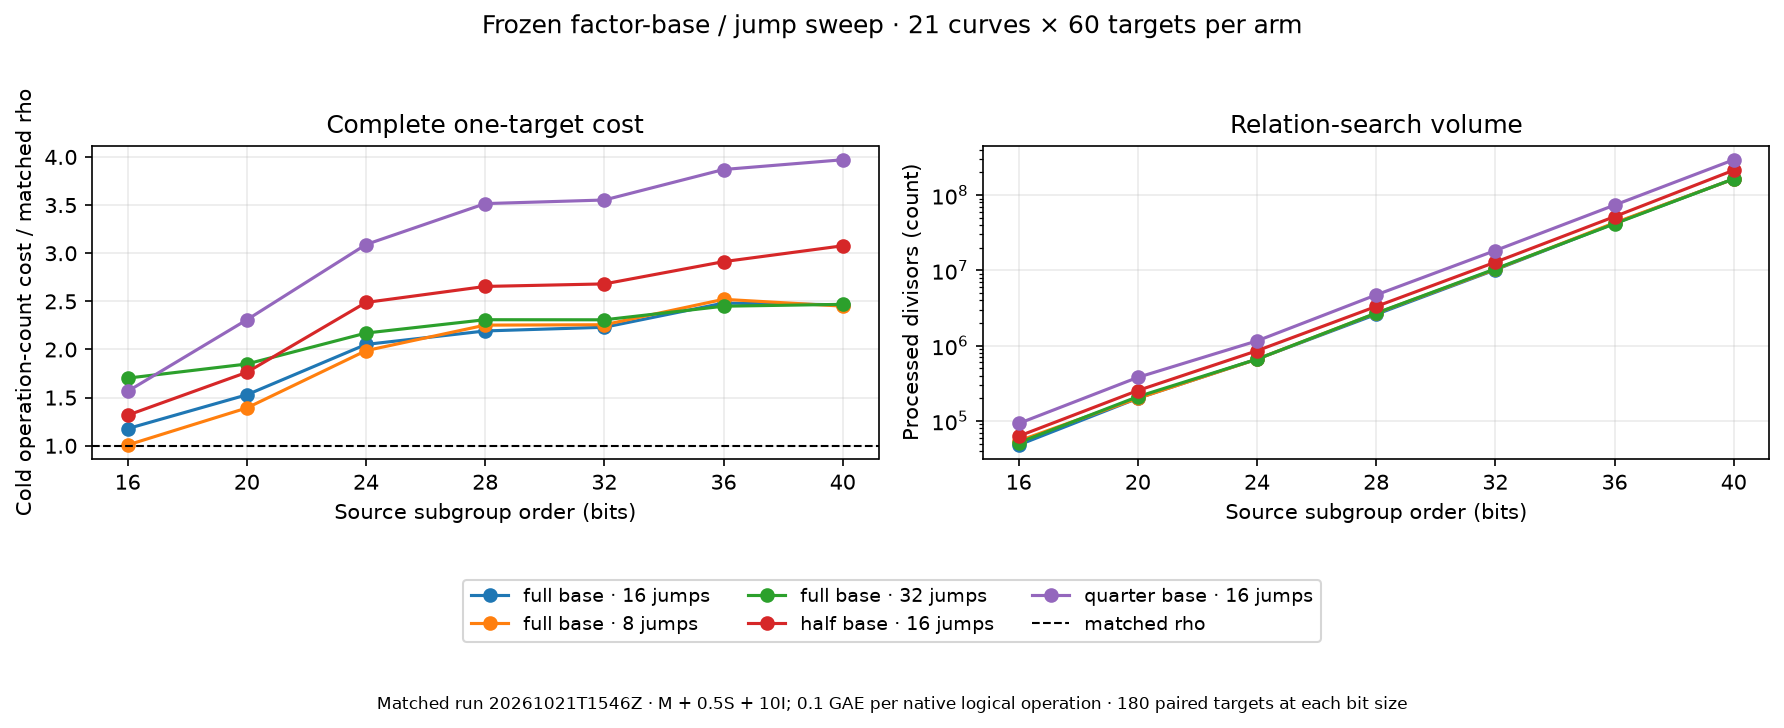
\includegraphics[width=0.98\linewidth]{factor-base-grid.png}
\end{center}

\clearpage
\section*{Kummer ordinary-addition gate}
Set $P=\tau(G)$ and $Q=2P$. The unsigned quotient gives $K(Q)=K(-Q)$,
but $K(P+Q)=K(3P)$ and $K(P-Q)=K(P)$ differ for order $r>4$.
The source-order, Jacobian-arithmetic and distinct-output checks passed on
21/21 exact-order models. This rules out binary ordinary addition from two
unsigned Kummer inputs for the current arbitrary-jump walk. A differential
walk with a known difference and sign/lift recovery has not been implemented
or priced.
\begin{center}
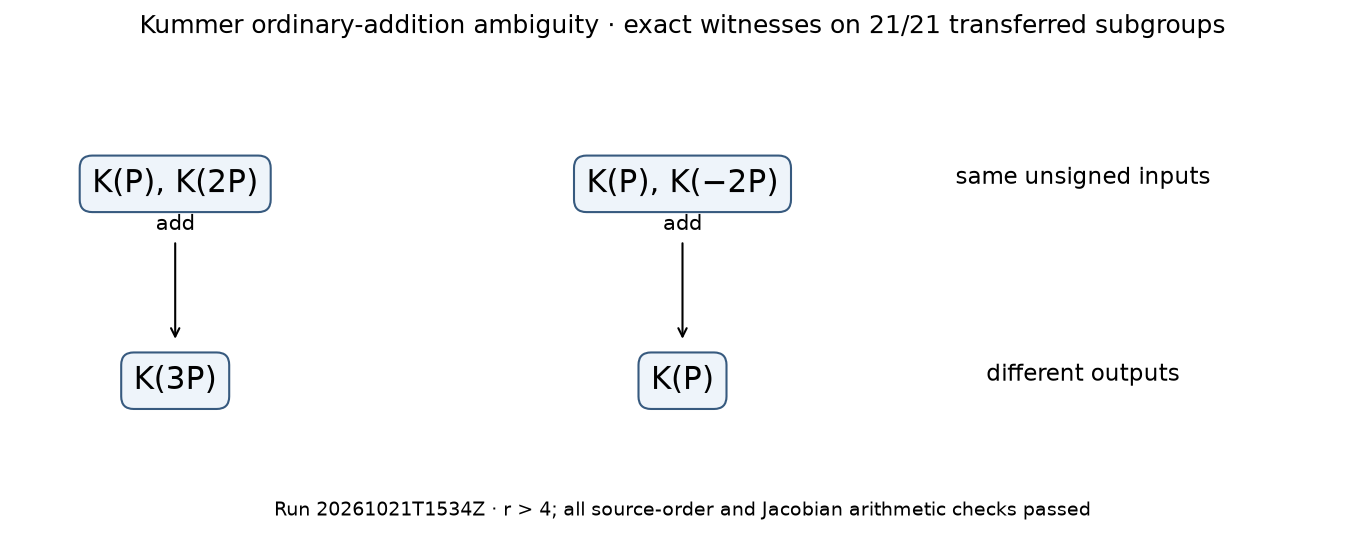
\includegraphics[width=0.86\linewidth]{kummer-ambiguity.png}
\end{center}

\section*{Open requirements and evidence}
The published complete inversion-free genus-2 formulas have not been
implemented or run on the 1,260 targets. The point-driven pencil collector
has a prior 20-target gate but no full-cohort result here. A differential
Kummer collector remains unimplemented. These are open requirements, not
negative end-to-end verdicts.

The machine record consists of 35 raw matched JSONL arm files, 6,300 paired
candidate/rho target rows, the full 36-cell price grid, summary JSON, 21
Kummer witnesses and a checksum manifest under
\path{research/four_followups_20261021/}.
The native analyzer pairs workload hashes, seeds, caps and source scalars;
the full-base arm reproduces the frozen external-law counts and phases. A
separate native validator recomputed 15 headline quantities from raw rows;
an archive-input rerun was compared byte-for-byte across all 35 files.
The plotting script only renders those recorded values. See
\url{https://github.com/aburan28/crypto/pull/2304} for the review branch and
\url{https://eprint.iacr.org/2024/623.pdf} for the separate complete-law path.
\end{document}
